\section{Fault-domain synthesis and probabilistic reliability}
\label{sec:reliability}
The same geometric certificate supports two different questions: whether every allowed failure is tolerated, and how often a target remains covered under a specified probability law. The first is adversarial and distribution-free. The second requires an actual distribution. Their numerical answers need not agree.

\subsection{Wiring as a hypergraph coloring problem}
Assign contact $i$ to a domain $g(i)\in\{1,\ldots,s\}$. A loss of a domain deletes all contacts assigned to it. For $A\in\mathcal A_T$, write $g(A)=\{g(i):i\in A\}$.

\begin{theorem}[Exact domain-design constraints]\label{thm:domain-design}
A domain assignment survives every loss of at most $q$ complete domains if and only if
\begin{equation}\label{eq:domain-design}
|g(A)|\ge q+1\quad\text{for every }A\in\mathcal A_T.
\end{equation}
The constraints are complete for the continuous target. If an assignment violates one, deleting its at most $q$ represented domains uncovers the associated witness point.
\end{theorem}
\begin{proof}
Apply \cref{thm:relabel} to the domain map. A domain contact set survives every loss of $q$ domains exactly when it has at least $q+1$ members, as in \cref{ex:domains}. \Cref{thm:universal} gives the equivalence and its failure witness.
\end{proof}

For $q=1$, the cut hypergraph must have no monochromatic edge. When all critical cuts have size two, this is ordinary proper graph coloring. Requiring every cut to contain every one of a specified set of colors is the familiar polychromatic or cover-decomposition formulation~\cite{polychromatic}. Equation \cref{eq:domain-design} allows more domains than the number of required surviving alternatives.

The finite constraints can be written as an integer program. Let $z_{ig}$ indicate assignment of contact $i$ to group $g$, and let $u_{Ag}$ indicate whether group $g$ occurs in cut $A$. Require
\[
\sum_g z_{ig}=1,\quad
u_{Ag}\ge z_{ig}\ (i\in A),\quad
u_{Ag}\le\sum_{i\in A}z_{ig},\quad
\sum_g u_{Ag}\ge q+1,
\]
with binary variables. The middle two constraints enforce the exact logical disjunction. A solver-proposed assignment can be checked directly against every certified cut; solver success alone is unnecessary for that verification. Proving that fewer groups are impossible requires a separate lower bound or exhaustive proof.

\begin{example}[An odd-cycle obstruction]\label{ex:oddcycle}
The three-asset geometry in \cref{sec:engineering} has critical patterns $\{1,2\},\{1,3\},\{2,3\}$. It is two-fold covered, but two domains cannot make every pair nonmonochromatic. Three domains suffice. Thus two-fold geometric coverage need not decompose into two separately covering domain layers. This is a finite example of the distinction studied in cover-decomposition theory, not a new general obstruction theorem.
\end{example}

\subsection{Ordinary target-coverage reliability}
Let $F$ now be a random failed-contact set. For ordinary coverage after that failure,
\begin{equation}\label{eq:random-success}
\mathbf1\{T\text{ remains covered}\}
=\prod_{A\in\mathcal A_T}\mathbf1\{A\not\subseteq F\}.
\end{equation}
The analogous formula for domain failures uses the mapped domain antichain. This is the standard minimal-cut representation of a semicoherent reliability system~\cite{barlow}. Some contacts may be irrelevant to the target; relevance of every component is not assumed.

If contacts fail independently with probabilities $p_i$, direct state enumeration gives
\begin{equation}\label{eq:reliability-enumeration}
\mathsf R(p)=\sum_{F\subseteq[n]}\left[\prod_{A\in\mathcal A_T}\mathbf1\{A\not\subseteq F\}\right]
\prod_{i\in F}p_i\prod_{i\notin F}(1-p_i).
\end{equation}
For cuts $A_1,\ldots,A_m$, inclusion--exclusion also gives
\begin{equation}\label{eq:reliability-ie}
\mathsf R(p)=\sum_{J\subseteq[m]}(-1)^{|J|}
\prod_{i\in\bigcup_{j\in J}A_j}p_i.
\end{equation}
The empty $J$ contributes one. Both formulas are exact and generally exponential; the geometric size bound does not turn arbitrary reliability evaluation into a polynomial-time algorithm.\footnote{A polynomial list of minimal cuts can still encode a difficult counting problem. The displayed three-contact calculation is a symbolic evaluation of four successful states, not an asymptotic algorithmic claim.}

For the odd-cycle example with identical independent failure probability $p$,
\[
\mathsf R(p)=(1-p)^3+3p(1-p)^2=1-3p^2+2p^3.
\]
The first equality enumerates the four mutually exclusive successful states, and its polynomial expansion gives the second equality directly.

\subsection{The same four sensors with two wiring choices}
For the four-corner panel, column wiring gives domain cuts $\{1\}$ and $\{2\}$: both domains must work. Diagonal wiring gives the single domain cut $\{1,2\}$: at least one domain must work. Under independent identical domain failure probability $p$,
\begin{equation}\label{eq:wiring-probability}
\mathsf R_{\mathrm{column}}=(1-p)^2,
\qquad
\mathsf R_{\mathrm{diagonal}}=1-p^2.
\end{equation}
At $p=1/10$ these are $81/100$ and $99/100$. The independent-failure law is a chosen model for this comparison. If the two domain failures are arbitrarily dependent but keep the same marginals $p$, the sharp two-event bounds are
\begin{align}
\max(0,1-2p)&\le\mathsf R_{\mathrm{column}}\le1-p,\label{eq:column-frechet}\\
1-p&\le\mathsf R_{\mathrm{diagonal}}\le\min(1,2-2p).\label{eq:diagonal-frechet}
\end{align}
They follow by writing the joint failure probability $a$ between $\max(0,2p-1)$ and $p$. Column success is $1-2p+a$, while diagonal success is $1-a$. At $p=1/10$, the intervals are $[4/5,9/10]$ and $[9/10,1]$.

The diagonal success event contains the column success event for every fixed domain-failure state. Thus its dominance under the same joint distribution does not require independence, even though the numerical values in \cref{eq:wiring-probability} do.

\subsection{Marginal-only reliability as a finite probability program}
If only marginal probabilities and selected dependence constraints are known, introduce a probability $\pi_F$ for each failure state. The sharp lower and upper coverage probabilities solve
\[
\min\text{ or }\max\quad\sum_F \pi_F\,\mathbf1\{A\not\subseteq F\text{ for all }A\in\mathcal A_T\}
\]
subject to $\pi_F\ge0$, $\sum_F\pi_F=1$, $\sum_{F\ni i}\pi_F=p_i$ and any stated additional linear probability constraints. This is the logical probability formulation of Hailperin~\cite{hailperin}, applied to the exact geometric cut list. It can have $2^n$ variables. No efficient solution for every dependence model is claimed.

\subsection{Maintaining a stronger residual requirement}
Equations \cref{eq:random-success,eq:kappa} concern ordinary coverage after a failure. If the desired residual rule is a different monotone predicate $w_0$, the exact condition is instead
\[
w_0(A\setminus F)=1\quad\text{for every }A\in\mathcal A_T.
\]
For nonnegative deletion costs, the exact attack cost becomes
\begin{equation}\label{eq:general-attack}
\min_{A\in\mathcal A_T}\ \min_{B\subseteq A:\,w_0(A\setminus B)=0}c(B).
\end{equation}
If some $A$ already loses under $w_0$, the inner minimum includes $B=\varnothing$ and the value is zero. Otherwise, a failure of an actual active set also fails a contained minimal active set, giving a no-more-expensive cut in that set; conversely that minimal set is realized at its witness. This proves \cref{eq:general-attack}.

For residual $k$-coverage at a pattern of size $a\ge k$, delete its $a-k+1$ cheapest contacts. A general $w_0$ may require a difficult inner optimization, and its complete minimal attack family can be much larger than $\mathcal A_T$. The universal geometric reduction remains exact without implying that every logical optimization is easy.

\begin{figure}[!htbp]
\centering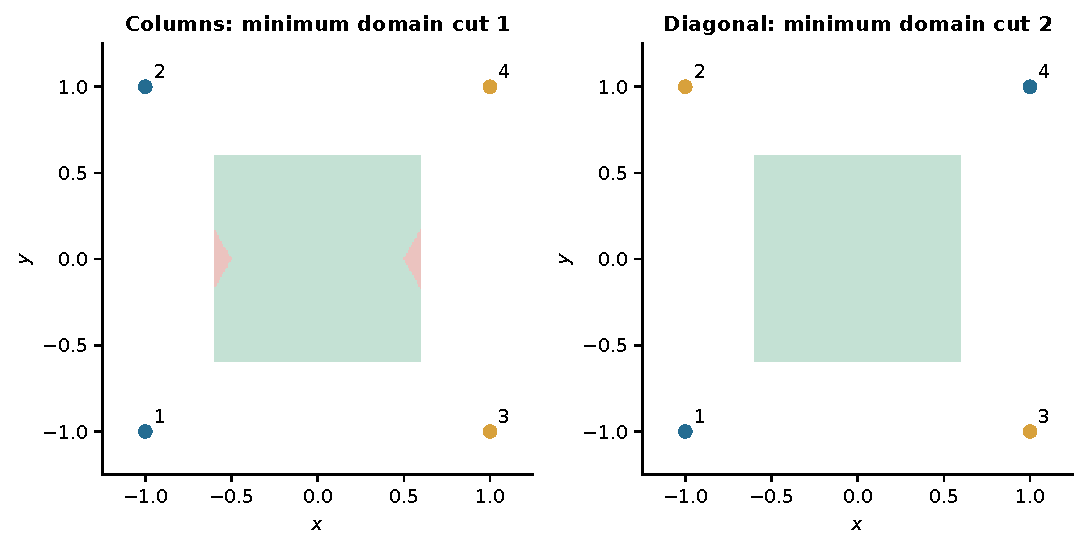
\includegraphics[width=\textwidth]{figures/wiring-comparison.pdf}
\caption{Wiring choices with the same geometry. The target shading illustrates whether two distinct domains are present. Exact certification gives the indicated minimum domain cuts. The geometric and stochastic conclusions use the separately stated models.}
\end{figure}

\begin{figure}[!htbp]
\centering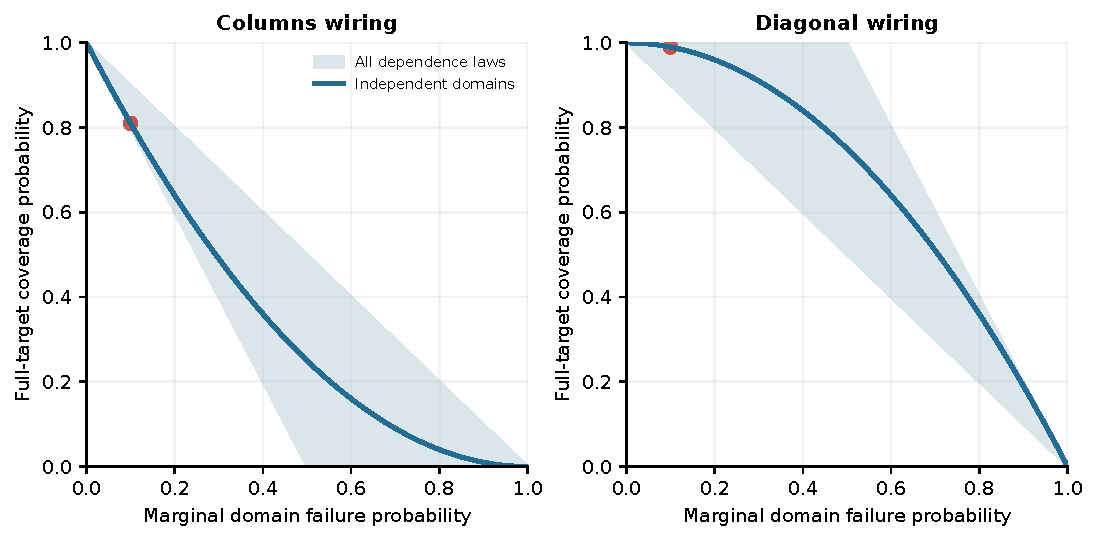
\includegraphics[width=\textwidth]{figures/reliability-curves.pdf}
\caption{Independent-domain reliability and sharp marginal-only bounds for the two wiring choices. The curves are the exact polynomials in \cref{eq:wiring-probability}; the shaded intervals allow arbitrary dependence with fixed marginals.}
\end{figure}

\FloatBarrier
